\documentclass[11pt,a4paper]{jsarticle}
%

\usepackage{amsmath,amssymb}
\usepackage{bm}
\usepackage[dvipdfmx]{color}
\usepackage[dvipdfmx]{graphicx}
\usepackage{ascmac}
\usepackage{listings, jlisting}
\lstset{%
  basicstyle={\small},%
  identifierstyle={\small},%
  commentstyle={\small\itshape},%
  keywordstyle={\small\bfseries},%
  ndkeywordstyle={\small},%
  stringstyle={\small\ttfamily},
  frame={tb},
  breaklines=true,
  columns=[l]{fullflexible},%
  numbers=none,%
  xrightmargin=0zw,%
  xleftmargin=3zw,%
  numberstyle={\scriptsize},%
  stepnumber=1,
  numbersep=1zw,%
  lineskip=-0.5ex%
}


%
\setlength{\textwidth}{\fullwidth}
\setlength{\textheight}{40\baselineskip}
\addtolength{\textheight}{\topskip}
\setlength{\voffset}{-0.2in}
\setlength{\topmargin}{0pt}
\setlength{\headheight}{0pt}
\setlength{\headsep}{0pt}

%
\newcommand{\divergence}{\mathrm{div}\,}  %ダイバージェンス
\newcommand{\grad}{\mathrm{grad}\,}  %グラディエント
\newcommand{\rot}{\mathrm{rot}\,}  %ローテーション
%
\title{チャレンジサイト・メカニックカモノハシ2019\\Ubuntu・Vimの基礎知識\\マイクロマウスシミュレータ導入}
\author{ER17045 立道壱太郎}
\date{\today}
\begin{document}
\maketitle
%
%
\section{この資料について}
メカニックカモノハシではマイクロマウス大会に参加することでメンバーの技術向上を図ります。
資料等はgithubに公開しているので、適時ダウンロードしてください。

\begin{lstlisting}[frame=single]
$ git clone https://github.com/platypus5384/micro_mouse.git
\end{lstlisting}

また、PC・Ubuntuの基本操作、vimの基本操作、プログラミング言語の基礎知識(if文・for文・配列等)が
多少(講義を受けた、1周間くらい使ったことがある程度)を想定しています。
最初は復習から始めますが、日常生活でも練習しておいてください。


\section{動作環境について}
Ubuntu16.04LTS

ROS Kinetic

での動作を前提としています。
Ubuntu18.04LTS等でも問題ないと思いますが、ros関連のパッケージ名が違ってくるので注意(kineticをmelodic等に変えるだけなので簡単)


\newpage

\section{Terminal及びVimの基礎知識}
Windowsは、ほとんどの作業をマウスで操作する事が出来ます(GUI,GraphicalUserInterface)。
Ubuntuでもマウス操作をすることが出来ますが、
基本的にはコマンド入力による操作(CUI,CharacterUserInterface 又はCLI,CommandLineInterface)が主になります。
慣れてくると、CUIの方が作業効率が良くなる(自由度が高く、scriptによる自動化も簡単に出来る)ので、これを機会に慣れましょう。

このセクションでは、Terminal及びVimを使うにあたって作業効率が格段に上がる基礎知識を紹介するので100%覚えましょう。
\subsection{Terminal}
デフォルトのTerminalを想定しています。
Terminator等では通用しないかもしれません。
\subsubsection{Terminalの開き方}
一応言っておくと、CtrlとAltはキーボード左下にあります。TはShiftキーを押さずにです。
\begin{lstlisting}[frame=single]
Ctrl + Alt + T
\end{lstlisting}

\subsubsection{Terminal内でのタブの開き方}
\begin{lstlisting}[frame=single]
Ctrl + Shift + T
\end{lstlisting}

\subsubsection{Terminal内でのタブ間の移動}
\begin{lstlisting}[frame=single]
Alt + [移動したいタブの左から数えた順番]
\end{lstlisting}

\subsubsection{Terminalの文字の大きさを変更する}
\begin{lstlisting}[frame=single]
Ctrl + Shift + 「+」
Ctrl + 「-」
\end{lstlisting}

\subsubsection{コマンド実行中に強制中断}
強制中断出来ない時もあります。
\begin{lstlisting}[frame=single]
Ctrl + C
\end{lstlisting}

\subsubsection{Terminalタブを閉じる}
タブが一個しかなければウィンドウを閉じます。
\begin{lstlisting}[frame=single]
Ctrl + D
\end{lstlisting}


\newpage

\subsection{Vim}
Vimとはエディタです。Vimの強みはCUI上で動くこと、自由度の高いコマンド操作です。

CUI上で作業できるのが強みという点は、のちのち理解できると思います。

Vimではコマンドを打つことで、コピペ、文字列置換やカーソル移動などが行えます。
また、Vimのコマンドはプログラムのような物で、自由度が高く使いこなせば作業効率が凄いことになるらしい。
プログラムを書く際には正直AtomやVisualStudioの方が便利ですが、
少し書く分には非常に便利で、また、どのPCにも基本的に入っているものなので、是非Vimに慣れましょう。

以下のサイトにわかりやすく載っていますが、量が多いので最低限これだけは、というのを紹介します。
使いながら覚えましょう。
\begin{lstlisting}[frame=single]
https://qiita.com/FBH9999/items/a8ec99bed08592a9d69a
\end{lstlisting}

\subsubsection{Vimのインストール}
Viというのはデフォルトで入っていますが、Vimはデフォルトで入っていせん。
ターミナル上で以下を実行してください。(\$を入力する必要はありません。\$から始まる行はターミナル上でという意味です。)
\begin{lstlisting}[frame=single]
$ sudo apt install vim
\end{lstlisting}

\subsubsection{Vimの起動}

\begin{lstlisting}[frame=single]
$ vim [ファイル名]
$ vim test.py        
$ vim (チュートリアルを開きます)
\end{lstlisting}

\subsubsection{編集モード}
編集モード(文章が書ける)に移行します。
\begin{lstlisting}[frame=single]
a (そのカーソル後から編集モードに)
i (そのカーソルから編集モードに)
\end{lstlisting}

\subsubsection{コマンドモード}
コマンドモードに移行します。
\begin{lstlisting}[frame=single]
Esc
又は、
Alt + コマンドの一文時目
\end{lstlisting}

\subsubsection{コマンド}
\begin{lstlisting}[frame=single]
:w (上書き保存)
:q (終了)
:!q (強制終了(保存せずに終了))
:wq (保存して終了)

:set number 行番号表示
:[数字] その行に移動


以下のコマンドは [数字] + コマンド とすることで一気にn回、n行できます。

h j k l それぞれ、左、下、上、右に移動(矢印でも移動できる)
u (1回作業を戻る (undo))
Ctrl + r (1回作業を進める (redo)
yy (1行コピー)
dd (1行コピー&削除)
p (ペースト)



\end{lstlisting}


\section{マイクロマウスパッケージの導入}
ROSが入っている、環境設定等が終わっている、というのを前提とします。(roscore出来れば問題なし)
\subsection{workspaceの作成}
メカニックカモノハシ用のworkspaceを新たに作りましょう。

\begin{lstlisting}[frame=single]
$ mkdir -p ~/mp_ws/src
$ cd ~/mp_ws/src/
$ catkin_init_workspace
$ echo "source ~/mp_ws/devel/setup.bash" >> ~/.bashrc
\end{lstlisting}


\subsection{マイクロマウスパッケージの導入}
githubから、パッケージをcloneしてcatkin\_makeします。
\begin{lstlisting}[frame=single]
$ cd ~/mp_ws/src
$ git clone https://github.com/platypus5384/micro_mouse.git
$ cd ~/mp_ws
$ catkin_ws
$ source ~/.bashrc
\end{lstlisting}

以下のコマンドを入力し、ディレクトリを移動できれば成功です。
\begin{lstlisting}[frame=single]
$ roscd micro_mouse
\end{lstlisting}


\newpage

\section{関連パッケージの導入}
マイクロマウスパッケージの動作に必要な関連パッケージを導入します。
以下のコマンドを実行してください。(全部で一行)
\begin{lstlisting}[frame=single, caption=roscd, label=roscd]
sudo apt install ros-kinetic-turtlebot ros-kinetic-turtlebot-msgs ros-kinetic-turtlebot-teleop 
\end{lstlisting}

\section{micro\_mouse動作テスト}
付いていると思いますが、一応、ファイルに権限を付けます。以下を実行してください。
\begin{lstlisting}[frame=single, caption=roscd, label=roscd]
$ roscd micro_mouse/script
$ sudo chmod -R a+x *
\end{lstlisting}

シミュレータを起動します。以下のコマンドをそれぞれ別端末で実行してください。
\begin{lstlisting}[frame=single, caption=roscd, label=roscd]
$ roslaunch micro_mouse startup.launch
別の端末を開き、
$ rosrun micro_mouse left_hund_ex.py
\end{lstlisting}


マウスが動き出し、マッピングが始まれば成功です。
しばらく待つと、以下のようになります。
\begin{figure}[h]
  \begin{center}
    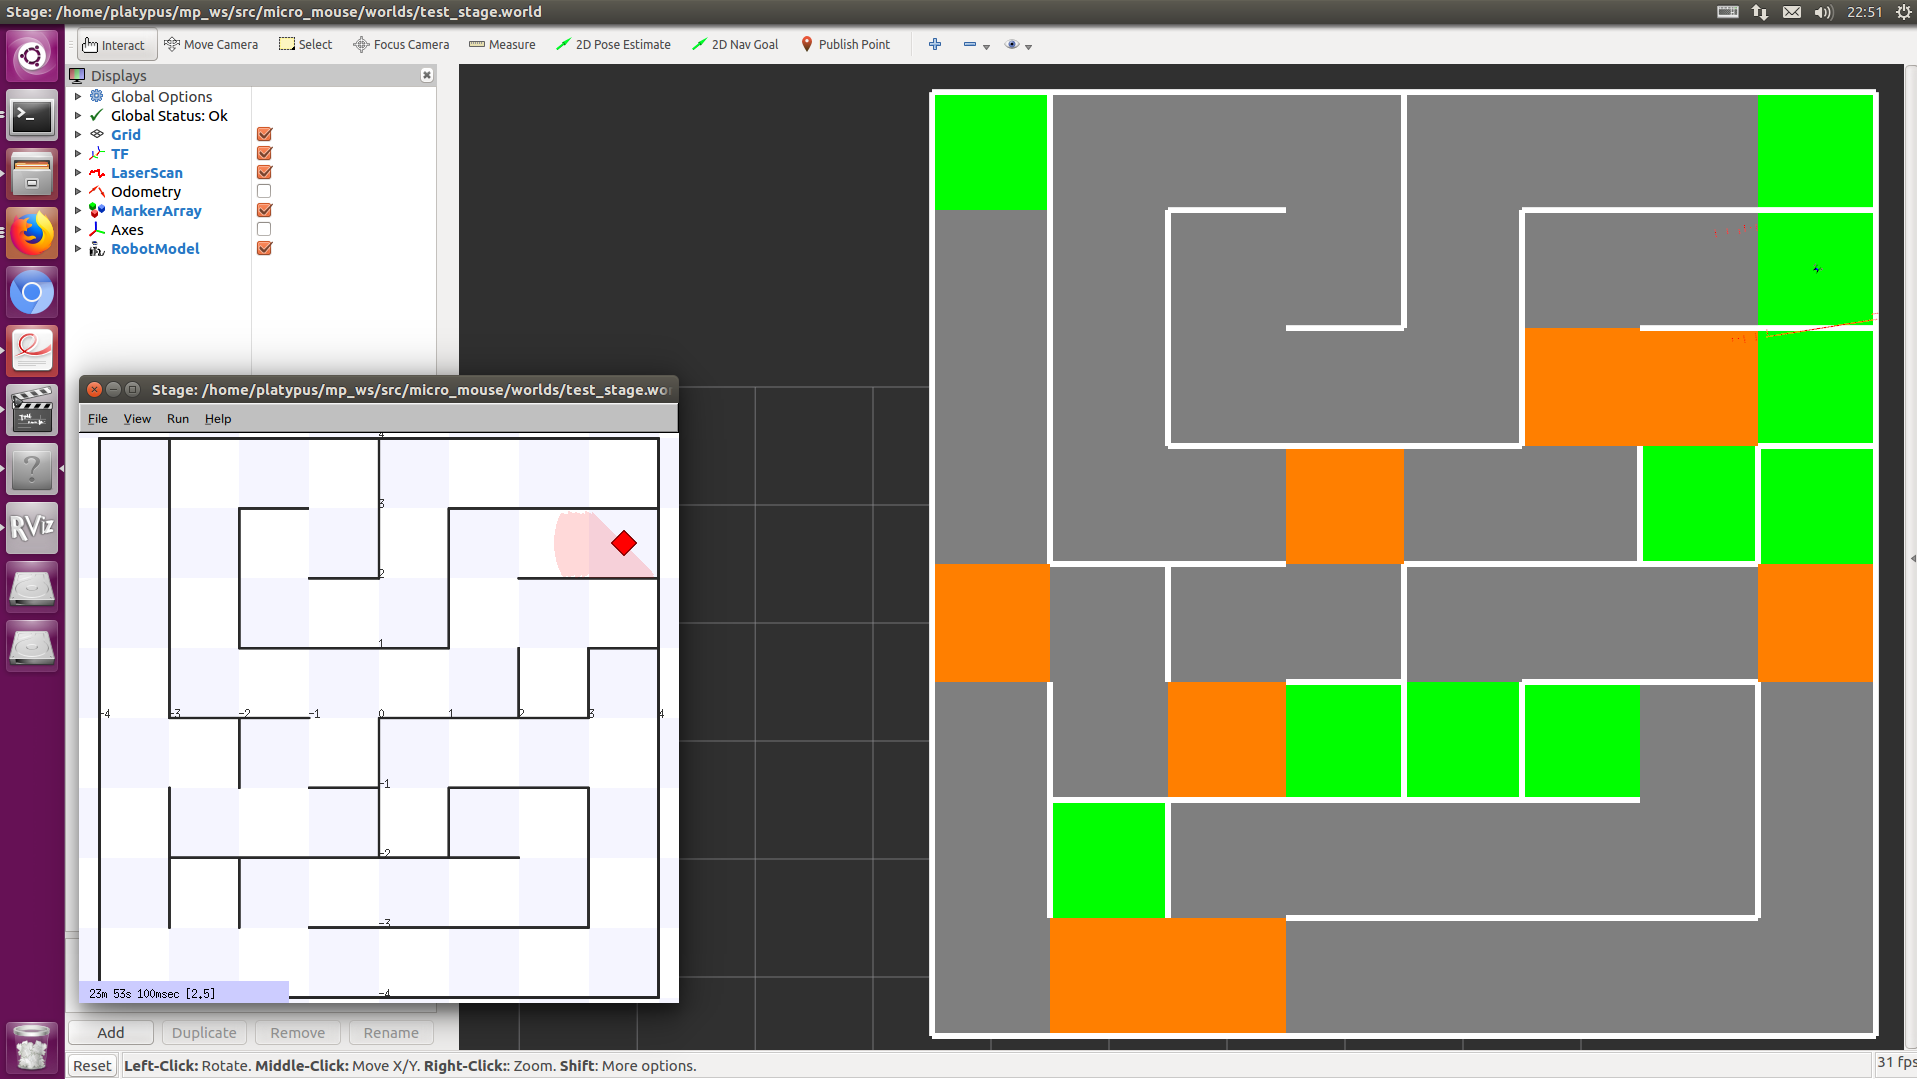
\includegraphics[width=128mm]{./mms_test.png}
  \end{center}
\end{figure}




\section{Exercise}
\subsection{Python簡易入門}
簡易的にPython入門しよう。

\newpage
\subsection{マウスを動かそう}

\lstinputlisting[caption=micro\_mouse/script/chapter/1/moving\_mouse.py,label=moveing_mouse,numbers=left]{./../../script/chapters/1/moving_mouse.py}


\newpage
\lstinputlisting[caption=micro\_mouse/script/chapter/1/going\_mouse.py,label=going_mouse,numbers=left]{./../../script/chapters/1/going_mouse.py}


\newpage
\lstinputlisting[caption=micro\_mouse/script/chapter/1/sensing\_mouse.py,label=sensing_mouse,numbers=left]{./../../script/chapters/1/sensing_mouse.py}




\newpage
\subsection{wallPublisherを使いこなそう}




\newpage
\subsection{pathPublisherを使いこなそう}




\newpage
\subsection{左手法・拡張左手法・足立法を理解しよう}
\subsubsection{左手法}
\lstinputlisting[caption=micro\_mouse/script/chapter/3/left\_hund.py,label=left_hund,numbers=left]{./../../script/chapters/3/left_hund.py}


\newpage
\subsubsection{拡張左手法}
\lstinputlisting[caption=micro\_mouse/script/chapter/3/left\_hund\_ex.py,label=left_hund_ex,numbers=left]{./../../script/chapters/3/left_hund_ex.py}


\subsubsection{足立法}





\newpage
\subsection{経路計画を理解しよう}



%\lstinputlisting[caption=moving\_mouse.py,label=moveing_mouse,numbers=left]{./../script/chapters/1/moving_mouse.py}


\begin{thebibliography}{99}
\bibitem{install_ubuntu16} Windows10とUbuntu16.04のデュアルブート環境構築\\https://qiita.com/medalotte/items/4bb5cfa709e93d044f1c
\bibitem{install_ubuntu18} Windows10とUbuntu18.04をデュアルブートする.\\https://qiita.com/yo\_kanyukari/items/2a944a300db22482c696
\end{thebibliography}%
%
\end{document}
